\documentclass[10pt,a4paper]{article}
\usepackage[margin=2.2cm]{geometry}
\usepackage{fontspec}
\usepackage{kotex}
\setmainfont{Apple SD Gothic Neo}
\setsansfont{Apple SD Gothic Neo}
\usepackage{amsmath,amssymb}
\usepackage{graphicx}
\usepackage{caption}
\usepackage[dvipsnames]{xcolor}
\usepackage[colorlinks=true,linkcolor=MidnightBlue,citecolor=MidnightBlue,
            urlcolor=MidnightBlue]{hyperref}
\usepackage{titlesec}
\titleformat{\section}{\large\bfseries}{\thesection}{0.6em}{}
\captionsetup{font=small,labelfont=bf}
\setlength{\parskip}{0.35em}
\setlength{\parindent}{0pt}
\usepackage{mdframed}
\newmdenv[linewidth=0.4pt,linecolor=gray!60,backgroundcolor=gray!5,
          innertopmargin=6pt,innerbottommargin=6pt,skipabove=8pt,skipbelow=8pt]{claimbox}
\newcommand{\claim}[2]{\begin{claimbox}\textbf{주장.} #1\par\smallskip
  \textcolor{gray!70}{\textbf{반증 조건.} #2}\end{claimbox}}

\title{\bfseries 정오: 배치 함수의 기제는 출력층이었다\\[2pt]
\large 논문 $201$ 의 \texttt{\_spec\_col} 주장 철회 --- 티처 \#$15$ 가 전송된 논문의 오류를 잡았다}
\author{월드모델 실험실 · 노트 $850$ 서문 (논문 $201$ 정오)}
\date{2026-08-09}
\begin{document}\maketitle

\section{한 줄}

논문 $201$ 은 ``$3$편 변경이 $27$편을 움직인'' 원인을 \texttt{\_spec\_col}
(배치 rankdata 피처)로 지목했다. \textbf{그 기제가 반증됐다}: spec 픽은
$12$씨앗 전수에서 `영화: None' 이고(재실측 --- venue 는 학습 $11$개 도메인이
관측해 \texttt{SPEC\_MAXDOM}$=4$ 를 넘으므로 원리상 픽 불가), 비회복
$27$행의 \textbf{설계행렬과 $32$자루 원점수가 두 팔에서 완전 동일}한데도
평균순위가 요동했다. 진짜 기제는 \textbf{출력층}(forms.py:$1080$) ---
predict 가 자루별 `배치 내 rankdata' 의 평균이라, 자루들이 어긋나는 근접짝은
삽입 위치가 자루마다 달라 평균이 뒤집힌다.

\begin{figure}[t]\centering
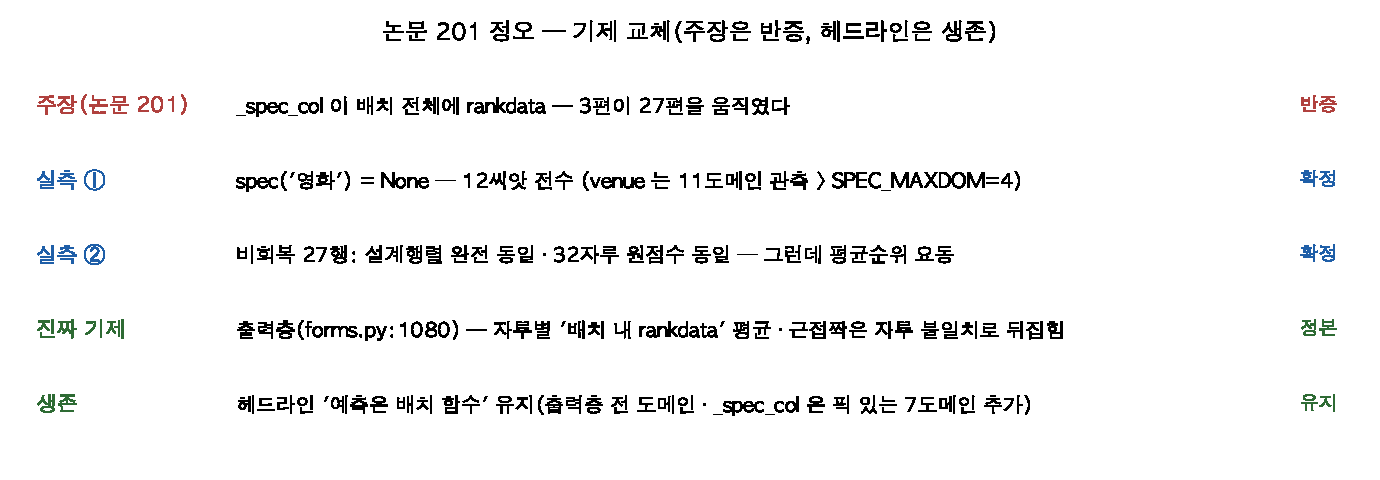
\includegraphics[width=0.97\textwidth]{figs/erratum.pdf}
\caption{정오 요약 --- 주장은 반증, 헤드라인은 생존.}
\end{figure}

\claim{\textbf{헤드라인('챔피언 예측은 배치 함수다')은 유지된다} --- 출력층은
전 도메인에 걸리고, \texttt{\_spec\_col} 은 픽이 있는 $7$개 도메인(아이돌 ·
게임 · 펀딩 · 웹툰 · 애니 · 모바일 · 세계애니)에서 추가로 걸린다. 그리고
$847$ 의 `삽입 캐스케이드' 해명은 이 실험에 한해 기제상 옳았다 --- $849$
에서 내가 철회한 것이 성급했고, `점수 불변 행의 짝 순서 보존' 은 \emph{모든
자루가 합의하는 짝}에만 성립하는 명제였다. 봉인 수확 채점(동결 순위 대 실현
라벨)은 배치 효과와 무관 --- 안전. 단 \textbf{판 채점의 배치 의존은
실재}한다(\texttt{\_score\_one} 이 라벨 결측 행까지 한 배치로 predict) ---
감사를 결정 규칙과 함께 T$1$ 미결로 등록했다.}
{부: 노트 $850$ 측정 --- 커버리지 결손 $+0.231$ 의 최종 주소는 정규화($+0.039$)도
사전 폭($3/9$ 회사 · 각 $1{\sim}2$편)도 아닌 \textbf{시장 꼬리의 극장 통계 밖
구조}($6$개 회사는 배급 필모가 있는데 pre-$2025$ 일별 표 대조 $0$). 순서 ·
문턱 예측은 $5$연속 적중대, 기제 서사는 계속 틀린다 --- 이 무늬 자체가
방법론이 됐다: \emph{효과의 크기와 기제는 걸지 말고, 순서와 문턱만 걸어라.}}

\end{document}
